\scanpage{12}

% 1, opening
Ens ordonné des cellules \deleted{\unsure{f.}} ouv. $X_i$

% 2–3, two lines of X terms
\diagram{\begin{tikzcd}[ampersand replacement=\&,row sep=tiny]
\bar X_{i-1}\arrow[d,dash]\\ X_{i-1}\quad X_i\&X_i
\end{tikzcd}}

% 4, heading
Géométrie des drapeaux de dim $\leq n$

% 5, examples
$D_0$ \uline{Ex} \qquad $n=0$\qquad $D_0$

% 6–7, first fork
\diagram{\begin{tikzcd}[ampersand replacement=\&,row sep=small,column sep=small]
n=1\&\&D_{01}\arrow[dl]\arrow[dr,"\text{\uline{épi} !!}"]\\
\&D_0\&\&D_1
\end{tikzcd}}

% 7–8, scratched repetition to the left
$\deleted{\bar X_{i-1}}\quad\deleted{X_{i-1}\ X_i}$ \quad $n=2$

% 8–10, three levels below the long line
\diagram{\begin{tikzcd}[ampersand replacement=\&,column sep=0.4em,row sep=small]
\&\& D_{012}\arrow[dl,dash]\arrow[d,dash]\arrow[dr,"\text{épi}",dash]\\
\&D_{01}\arrow[dl,dash]\arrow[dr,"\text{épi}"']\&D_{02}\arrow[dll,dash]\arrow[drr,dash]\&D_{12}\arrow[dl,dash]\arrow[dr,"\text{épi}",dash]\\
 D_0\&\&D_1\&\&D_2
\end{tikzcd}}

% 8–10, right of the triangle
$D_{01\ldots i}\to D_I$ \uuline{épi} si $i=\operatorname{Sup} I$ i.e. $i\in I\subset[0,i]$

% 11, central label
$D_I$

% 12–15, central fork with F labels
\diagram{\begin{tikzcd}[ampersand replacement=\&,row sep=small,column sep=.5em]
\&\&D_{012}(F)\arrow[ddl,dash]\arrow[d]\arrow[dr,"\text{épi}"]\\
\&\&D_{02}(F)\arrow[ddll,dash,bend left=15]\arrow[ddrr,dash,bend right=10]\&D_{12}(F)\arrow[ddl,bend right=12]\arrow[ddr,"\unsure{e}"]\\
\&D_{01}\arrow[dl,dash]\arrow[dr]\\
D_0\&\&D_1\&\&\unsure{\{M\}|\{m\}|\{1\}}
\end{tikzcd}}

% 12–14, separate square at right
\diagram{\begin{tikzcd}[ampersand replacement=\&,row sep=small,column sep=small]
D_{012}\arrow[r]\arrow[d]\&D_{12}\arrow[d,dash]\\
D_{02}\arrow[r]\&D_2
\end{tikzcd}}

% 14–16, left-hand scratch
\diagram{\begin{tikzcd}[ampersand replacement=\&,row sep=tiny,column sep=small]
j\quad j{+}1\&D_{123}\arrow[d]\\
\deleted{D_{j\ldots j}}\&D_{13}\\
\&\overline{D_{13}}
\end{tikzcd}}

% 15–16, central bracket
\figure{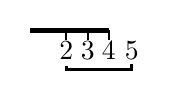
\begin{tikzpicture}[scale=.65]\draw[line width=2pt](-.7,.28)--(.83,.28); \foreach \x in {0,.42,.83}{\draw[thick](\x,.28)--(\x,.1);} \foreach \x/\v in {0/2,.42/3,.83/4,1.28/5}{\node at (\x,-.12){$\v$};} \draw[very thick](0,-.41)--(0,-.48)--(1.28,-.48)--(1.28,-.38);\end{tikzpicture}}

% 15–16, pair of intervals at right
\figure{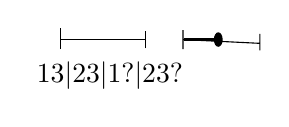
\begin{tikzpicture}[scale=.8]\draw (0,0)--(1.35,0) (0,-.15)--(0,.18) (1.35,-.14)--(1.35,.13); \node at (.78,-.57){$\unsure{13|23|1?|23?}$}; \draw(1.94,0)--(3.16,-.06) (1.94,-.15)--(1.94,.15) (3.16,-.17)--(3.16,.09); \draw[very thick](1.95,0)--(2.5,0);\fill(2.5,0)ellipse(.07 and .115);\end{tikzpicture}}

% 17–20, left repeated triangle
\diagram{\begin{tikzcd}[ampersand replacement=\&,column sep=0.4em,row sep=small]
\&\& D_{012}\arrow[dl,dash]\arrow[d,very thick,dash]\arrow[dr,"\text{épi}",dash]\\
\&D_{01}\arrow[dl]\arrow[dr,"\text{épi}"']\&D_{02}\arrow[dll,dash]\arrow[drr,dash]\&D_{12}\arrow[dl,dash]\arrow[dr,"\text{épi}",dash]\\
 D_0\&\&D_1\&\&D_2
\end{tikzcd}}

% 17–21, right-hand criterion
$D_\sigma\unsure{-|\to}D_{\sigma'}$ épi \uline{si} $\sigma'\subset\sigma$ est segment final de $\sigma$ i.e. $\sigma=\sigma''\cup\sigma'$ avec $\sigma''<\sigma'$

% 17, isolated mark above the lower diagram
$\unsure{7|\urcorner}$

% 19–24, large diagram
\diagram{\begin{tikzcd}[ampersand replacement=\&,row sep=small,column sep=0.05em]
\&\&\&\&\&\&D_{0123}\arrow[dlll]\arrow[d]\arrow[dr,very thick]\\
\&\&\&D_{013}\arrow[ddll,bend right=20]\arrow[dr]\arrow[drr,very thick]\&\&\&D_{023}\arrow[dll,dashed]\arrow[dr,very thick]\&D_{123}\arrow[dll]\arrow[d,very thick]\\
\&\&D_{012}\arrow[dl,dashed]\arrow[d]\arrow[dr,very thick,"\text{épi}"]\arrow[dd,bend left=65]\arrow[rr,dash]\&\&D_{03}\arrow[ddr,very thick]\&D_{13}\arrow[dd,very thick]\&\&D_{23}\arrow[ddll,very thick]\\
\&D_{01}\arrow[dl]\arrow[d,very thick]\&D_{02}\arrow[dll,dashed]\arrow[d,very thick]\&D_{12}\arrow[dll,dashed]\arrow[dl,very thick,"\text{épi}"]\\
D_0\&D_1\&D_2\&\&\&D_3
\end{tikzcd}}

% 25–28, two columns at foot
\[
\begin{aligned}
D_{01}&\mathbin{-}D_1 &D_{013}&\mathbin{-}D_{13}\\
D_{012}&\to D_{12} &D_{0123}&\mathbin{-}D_{123}\\
D_{12}&\mathbin{-}D_2 &D_{123}&\mathbin{-}D_{23}\\
D_{02}&\mathbin{-}D_2 &D_{23}&\mathbin{-}D_3
\end{aligned}
\]

% bottom right, ruled wedge with indices
\figure{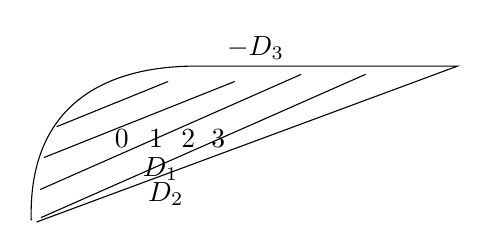
\begin{tikzpicture}[x=.95cm,y=.7cm]\draw (0,0)..controls (-.04,2) and (.9,2.8)..(2.21,2.8)--(5.7,2.8)--(.07,-.03); \draw (.34,1.7)--(1.83,2.52) (.17,1.14)--(2.72,2.52) (.12,.56)--(3.61,2.65) (.13,.05)--(4.47,2.65); \node at (3,3.12){$-D_3$}; \foreach \x/\v in {1.21/0,1.67/1,2.1/2,2.5/3}{\node at (\x,1.48){$\v$};} \node at (1.73,.93){$D_1$}; \node at (1.8,.48){$D_2$};\end{tikzpicture}}

% bottom, numerical working
\[
\begin{aligned}
&1\quad 1+1\quad 1+2+\\[-1pt]
&\hspace{3em}\shortparallel\\[-1pt]
 n_i&=\sum_{j<i}n_j+1\qquad 2
\end{aligned}
\]

% lower left
% archive sheet number: 11
